% !TEX TS-program = xelatex
\documentclass[12pt,letterpaper]{article}
\usepackage{amsmath,amssymb}
\usepackage{fontspec}
\setmainfont{EB Garamond}[Numbers=OldStyle,Ligatures=TeX]
\usepackage{tikz}
\usetikzlibrary{calc,positioning,arrows.meta,fit,backgrounds,shapes.geometric}
\usepackage[letterpaper,margin=1in]{geometry}
\usepackage{caption}

\begin{document}

\section*{Option 1: Minimal DAG (6 nodes)}

\begin{figure}[h]
\centering
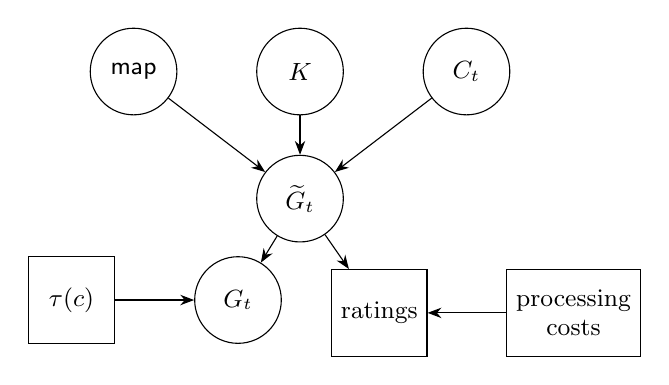
\begin{tikzpicture}[
  %node distance=0.5cm and 2.2cm,
  latent/.style={draw,circle,minimum size=1.1cm,font=\small},
  observed/.style={draw,rectangle,minimum size=1.1cm,font=\small},
  every edge/.style={draw,-{Stealth[length=5pt]}},
]
  % State layer
  \node[latent] (map) {$\mathsf{map}$};
  \node[latent,right=of map] (K) {$K$};
  \node[latent,right=of K] (Ct) {$C_t$};

  % Stability score
  \node[latent,below=0.5cm of K] (Gtilde) {$\widetilde{G}_t$};

  % Membership
  \node[latent,below left=0.5cm and 0cm of Gtilde] (Gt) {$G_t$};
  \node[observed,left=of Gt] (tau) {$\tau(c)$};

  % Observation
  \node[observed,below right=0.5cm and 0cm of Gtilde] (ratings) {ratings};
  \node[observed,right=of ratings] (proc) {\shortstack{processing\\costs}};

  % Edges: state
  \path (map) edge (Gtilde);
  \path (K) edge (Gtilde);
  \path (Ct) edge (Gtilde);

  % Edges: threshold
  \path (Gtilde) edge (Gt);
  \path (tau) edge (Gt);

  % Edges: observation
  \path (Gtilde) edge (ratings);
  \path (proc) edge (ratings);
\end{tikzpicture}
\caption*{\textbf{Option 1: Minimal.} Circles = latent; rectangles = observed/set. Ratings reflect $\widetilde{G}_t$ plus processing costs, not $G_t$ directly.}
\end{figure}

\clearpage
\section*{Option 2: Medium DAG (11 nodes)}

\begin{figure}[h]
\centering
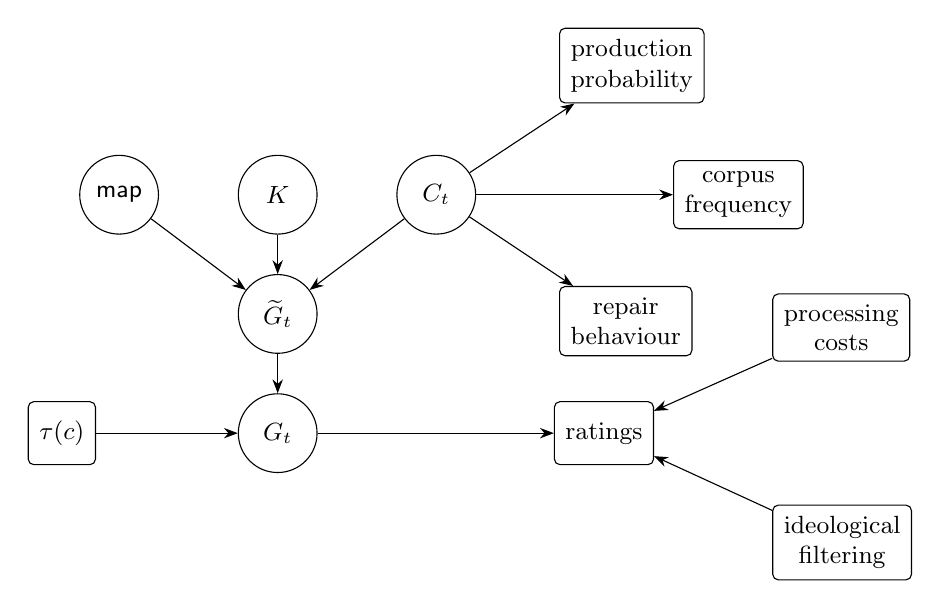
\begin{tikzpicture}[
  %node distance=1.6cm and 2cm,
  latent/.style={draw,circle,minimum size=1cm,font=\small},
  observed/.style={draw,rectangle,rounded corners=2pt,minimum height=0.8cm,font=\small,inner sep=4pt},
  every edge/.style={draw,-{Stealth[length=5pt]}},
]
  % State layer
  \node[latent] (map) {$\mathsf{map}$};
  \node[latent,right=of map] (K) {$K$};
  \node[latent,right=of K] (Ct) {$C_t$};

  % Stability score
  \node[latent,below=0.5cm of K] (Gtilde) {$\widetilde{G}_t$};

  % Membership
  \node[latent,below=0.5cm of Gtilde] (Gt) {$G_t$};
  \node[observed,left=1.8cm of Gt] (tau) {$\tau(c)$};

  % Observation layer
  \node[observed,right=3cm of Gt] (ratings) {ratings};
  \node[observed,above right=0.5cm and 1.5cm of ratings] (proc) {\shortstack{processing\\costs}};
  \node[observed,below right=0.5cm and 1.5cm of ratings] (ideo) {\shortstack{ideological\\filtering}};

  % C_t indicators (above and right of C_t)
  \node[observed,above right=0.8cm and 1.2cm of Ct] (prod) {\shortstack{production\\probability}};
  \node[observed,right=2.5cm of Ct] (corpus) {\shortstack{corpus\\frequency}};
  \node[observed,below right=0.8cm and 1.2cm of Ct] (repair) {\shortstack{repair\\behaviour}};

  % Edges: state
  \path (map) edge (Gtilde);
  \path (K) edge (Gtilde);
  \path (Ct) edge (Gtilde);

  % Edges: threshold
  \path (Gtilde) edge (Gt);
  \path (tau) edge (Gt);

  % Edges: observation (ratings)
  \path (Gt) edge (ratings);
  \path (proc) edge (ratings);
  \path (ideo) edge (ratings);

  % Edges: C_t indicators (C_t causes the observations)
  \path (Ct) edge (prod);
  \path (Ct) edge (corpus);
  \path (Ct) edge (repair);
\end{tikzpicture}
\caption*{\textbf{Option 2: Medium.} Adds $C_t$'s observable indicators (right) and ideological filtering. $C_t$ is latent, inferred from converging evidence.}
\end{figure}

\clearpage
\section*{Option 3: Full DAG - polished}

\begin{figure}[h]
\centering
\def\BoxH{1.2cm} % ratings box height
\def\RowSep{1.7cm} % main-row centre-to-centre distance (= BoxH + 0.5cm gap)
\def\HalfRow{0.85cm} % half-row offset (between main rows)
\def\Col{2.7cm} % main column spacing
\def\Branch{2.6cm} % separation between ratings and production probability
\def\Dx{0.5cm} % slight right-offset for half-row nodes

\begin{tikzpicture}[
  % Single-stroke circles for latent variables
  latent/.style={circle, draw, line width=0.6pt,
    minimum size=\BoxH, font=\normalsize, inner sep=0pt},
  % Rounded rectangles for observed/set quantities
  observed/.style={rectangle, rounded corners=5pt, draw,
    line width=0.6pt, minimum height=\BoxH, minimum width=1.9cm,
    font=\small, inner sep=6pt, align=center},
  % Diamonds for conditioning anchors
  cond/.style={diamond, draw, line width=0.6pt, minimum size=\BoxH,
    font=\normalsize, inner sep=3pt, align=center},
  % Thin arrows with small heads
  every edge/.style={draw, line width=0.5pt, -{Stealth[length=4pt, width=3pt]}},
]

  % === Row baselines (5 main rows) ===
  \coordinate (r1) at (0,0);
  \path (r1) ++(0,-\RowSep) coordinate (r2);
  \path (r2) ++(0,-\RowSep) coordinate (r3);
  \path (r3) ++(0,-\RowSep) coordinate (r4);
  \path (r4) ++(0,-\RowSep) coordinate (r5);

  % === Column baselines (main block) ===
  \coordinate (c1) at (0,0);
  \path (c1) ++(\Col,0) coordinate (c2);
  \path (c2) ++(\Col,0) coordinate (c3);
  \path (c3) ++(\Col,0) coordinate (c4);

  % === Row 1: Conditioning ===
  \node[observed] (stakes) at (c1 |- r1) {stakes};
  \node[cond] (S) at (c2 |- r1) {$S$};
  \node[cond] (A) at (c3 |- r1) {$A$};
  \node[cond] (I) at (c4 |- r1) {$I$};

  % === Row 2: c ===
  \node[latent] (c) at (c3 |- r2) {$c$};

  % === Row 3: State variables + threshold ===
  \node[observed] (tau) at (c1 |- r3) {$\tau(c)$};
  \node[latent] (map) at (c2 |- r3) {$\mathsf{map}$};
  \node[latent] (K) at (c3 |- r3) {$K$};
  \node[latent] (Ct) at (c4 |- r3) {$C_t$};

  % === Row 4: Stability score + observation row ===
  \node[latent] (Gtilde) at (c3 |- r4) {$\widetilde{G}_t$};

  % Left edge of ratings aligned with left edge of C_t
  \node[observed,anchor=west] (ratings) at ($(Ct.west)+(0,-\RowSep)$) {ratings};

  % C_t indicator aligned to the same row as ratings
  \node[observed,anchor=west] (prod) at ($(ratings.east)+(\Dx,2*\RowSep)$) {\shortstack{production\\probability}};

  % === Half-row nodes (between the 5 main rows) ===
  \node[observed,anchor=west] (proc) at ($(ratings.east)+(\Dx,0)$) {\shortstack{processing\\costs}};
  \node[observed,anchor=west] (ideo) at ($(ratings.east)+(\Dx,-\RowSep)$) {\shortstack{ideological\\filtering}};

  \node[observed,anchor=west] (corpus) at ($(prod.west)+(0,\RowSep)$) {\shortstack{corpus freq.\\/\,opportunity}};
  \node[observed,anchor=west] (repair) at ($(prod.west)+(0,-\RowSep)$) {\shortstack{repair\\behaviour}};

  % === Row 5: Membership ===
  \node[latent] (Gt) at (c3 |- r5) {$G_t$};

  % === Edges: conditioning ===
  \path (S) edge (c);
  \path (A) edge (c);
  \path (I) edge (c);
  \path (stakes) edge (tau);
  \path (c) edge (tau.north east);

  % === Edges: c → state variables ===
  \path (c) edge (map);
  \path (c) edge (K);
  \path (c) edge (Ct);

  % === Edges: state → stability ===
  \path (map) edge (Gtilde);
  \path (K) edge (Gtilde);
  \path (Ct) edge (Gtilde);

  % === Edges: threshold → membership ===
  \path (Gtilde) edge (Gt);
  \path (tau) edge (Gt);

  % === Edges: observation (from G̃_t, NOT G_t) ===
  \path (Gtilde) edge (ratings);
  \path (proc) edge (ratings);
  \path (ideo) edge (ratings);

  % === Edges: C_t → indicators (all direct from C_t) ===
  \path (Ct) edge (prod);
  \path (Ct) edge (corpus.south west);
  \path (Ct) edge (repair);
\end{tikzpicture}
\caption*{\textbf{Option 3 (polished).} Circles\,=\,latent; rounded rectangles\,=\,observed/set; diamonds\,=\,conditioning anchors. Ratings are downstream of $\widetilde{G}_t$ (stability), not $G_t$ (membership). $C_t$ indicators are each direct outputs of $C_t$.}
\end{figure}

\end{document}
